\section{Implementation}

\subsection{System Architecture}
The architecture of the system we proposed can be seen in
figure \ref{system-architecture}.
We can separate the deployment into 4 groups.
\begin{enumerate}
      \item The first one, the ESP32, are the physical device
            that gathers the air quality data and controls the door.
      \item Second, the Application Server are the primary brain
            of the whole system from collecting the data
            retrieved from the ESP32, saving the data, to
            managing the state of the system.
      \item Third, the SparkMachine, are the processor of data
            that processes the data into more meaningful
            informations for the user, such as minimum, maximum,
            and average values.
      \item Lastly, the User Device are users' devices that
            accesses the web application to interact with the
            system.
\end{enumerate}

\begin{figure*}
      \centering
      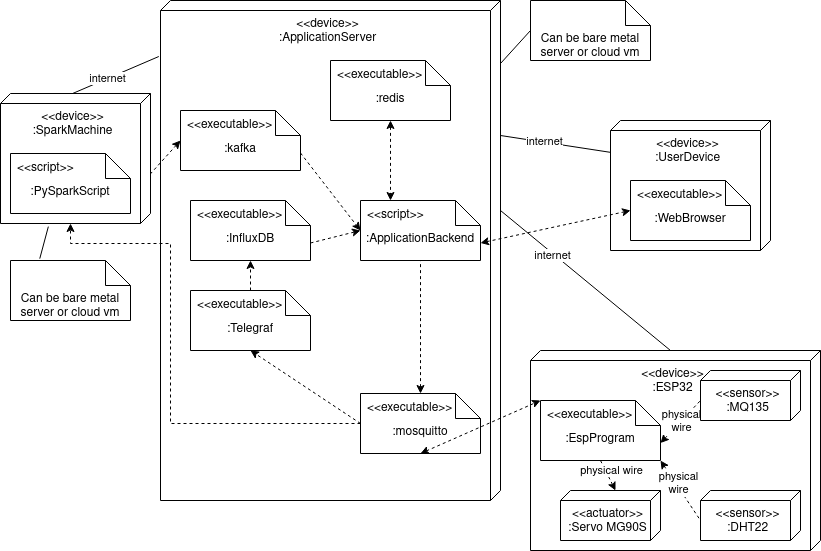
\includegraphics[scale=0.5]{resources/deployment-diagram.png}
      \caption{Deployment diagram of the smart room air conditioner}
      \label{system-architecture}
\end{figure*}

\begin{figure}
      \centering
      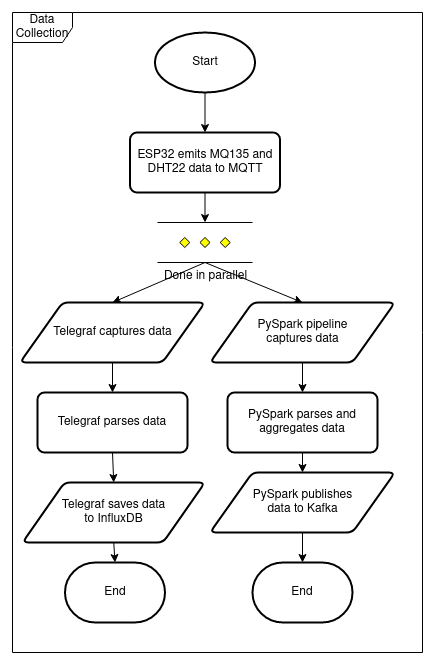
\includegraphics[scale=0.44]{resources/flowchart-data-collection.png}
      \caption{Flowchart of the data collection in the system}
      \label{flowchart-data-collection}
\end{figure}

\begin{figure}
      \centering
      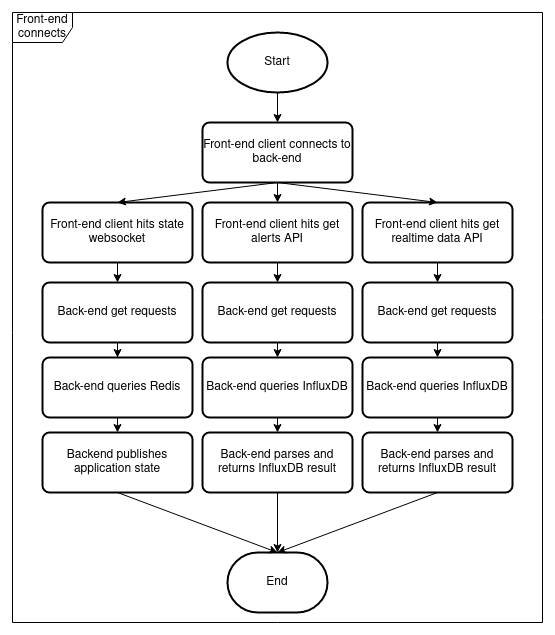
\includegraphics[scale=0.44]{resources/flowchart-fe-connects.png}
      \caption{Flowchart of the system when the front-end connects to the back-end}
      \label{flowchart-fe-connects}
\end{figure}

\begin{figure}
      \centering
      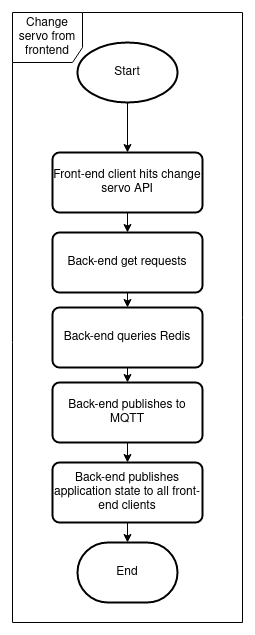
\includegraphics[scale=0.44]{resources/flowchart-fe-change-servo.png}
      \caption{Flowchart of the system when the front-end hits the change servo API}
      \label{flowchart-fe-change-servo}
\end{figure}

\begin{figure}
      \centering
      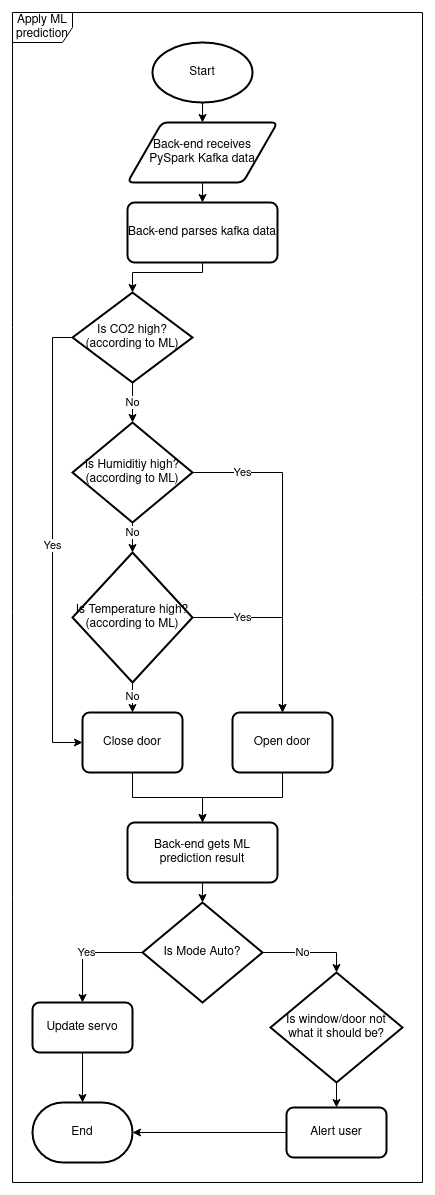
\includegraphics[scale=0.44]{resources/flowchart-apply-ml.png}
      \caption{Flowchart of the machine learning application in the system}
      \label{flowchart-apply-ml}
\end{figure}

Flow-wise, as we can see in the figure
\ref{flowchart-data-collection} the data gathered
by the MQ135 and DHT22, in the ESP32, are emitted
to the mosquitto, the MQTT broker. There, the data
are captured by both Telegraf and by PySpark
pipeline. The Telegraf then parses the data and
saves the data into the InfluxDB. While the PySpark
pipeline parses the data and applies aggregation
functions to get aggregate values such as minimum,
maximum, median, and average values. The aggregate
values are then published into the Kafka, to be
consumed by the Application Server.

The Application Server then consumes the data from
the InfluxDB and the Kafka. The figure
\ref{flowchart-fe-connects} shows the flow when the
front-end connects to the back-end. When the
front-end calls the realtime data API, the back-end
will receive the requests, then queries and parses
the data that have been saved into the InfluxDB to
be displayed by the front-end.
So does the flow when the front-end calls the
alerts API, the back-end will receive the requests,
then queries and parses the data from InfluxDB, but this time to get alerts data.

In the event of the front-end calls the state
websocket, the back-end will parses the data,
queries the current state from the Redis, and
publishes the current state to the connected
front-end client.

Still in the Web Application part, the figure
\ref{flowchart-fe-change-servo} shows the flow when
the front-end calls the change servo API. When the
front-end calls the change servo API, the back-end
will receive the requests, then queries the current
state from the Redis, and publishes the new state
to the MQTT to be consumed by the ESP32. The back-end will then publishes the new state to all connected front-end clients via websocket.

The figure \ref{flowchart-apply-ml} shows the flow
of the implementation of the machine learning
model in the system. Every time the back-end receives
the aggregate values from the Kafka, the back-end
will then parses and passes the data to the machine
learning models. The machine learning models will
then determine the current air quality level of
each indicators. The system then determines whether
the door should be opened or closed based on the
current air quality level of each indicators and
the rules defined. If the CO$_2$ ppm is high, the
door should be closed. If the CO$_2$ ppm is low,
and the temperature or humidity are high, the door
should be opened. If all the indicators are low,
the door should be closed.

\subsection{Machine Learning Model}
Since the data gathered by the sensors are time
series data, we will use Time Series KMeans (TSKM)
algorithm to cluster the data, that is provided in
python by
\href{https://tslearn.readthedocs.io/en/stable/}{\texttt{tslearn}} library.
KMeans algorithm are chosen because it is simple and
easy to implement, and it is also one of the most
popular clustering technique.

To train the model, we used the data gathered by the
sensors for 3 days, as the InfluxDB database stores,
from 2021-05-01 to 2021-05-03. Since the data,
especially from the MQ135 sensor were not too
accurate, we ``smoothened'' the data by using the
\href{https://pandas.pydata.org/docs/reference/api/pandas.DataFrame.rolling.html}{\texttt{rolling}} mean, which saves
the mean of the current rolling window of 120 data. The number
120 is chosen arbitarily to ensure the data is smooth enough,
but not too smooth that it loses its meaning. We also used 2
clusters for the model, as we only need to separate the data
into ``good'' and ``bad'' air quality.

The result of the training can be seen in
figure \ref{kmeans}. Due to use of clustering algorithm, we could not
determine the exact value of each indicators that is the
discriminant point that separates the ``good'' and ``bad''
air quality, but we can see that the ``good'' air quality is
represented by the lower part, and the ``bad'' air quality is
represented by the upper part.

We then implement the model into the system by passing each
indicator's current average value to the model to determine
the current air quality level of the room. The result of the
model is then used to determine whether the door should be
opened or closed using the following rules:
\begin{enumerate}
      \item If the CO$_2$ level is ``bad'', the door will not be
            opened, since we don't want any toxic particles to
            get in the room.
      \item If the CO$_2$ level is ``good'', we will check the
            next indicators, temperature and humidity. If
            either temperature or humidity is ``bad'', then the
            door will be opened, since we want to get fresh
            air into the room.
      \item If both temperature and humidity are ``good'',
            then the door will not be opened, since the air
            quality is already good.
\end{enumerate}

\begin{figure}
      \centerline{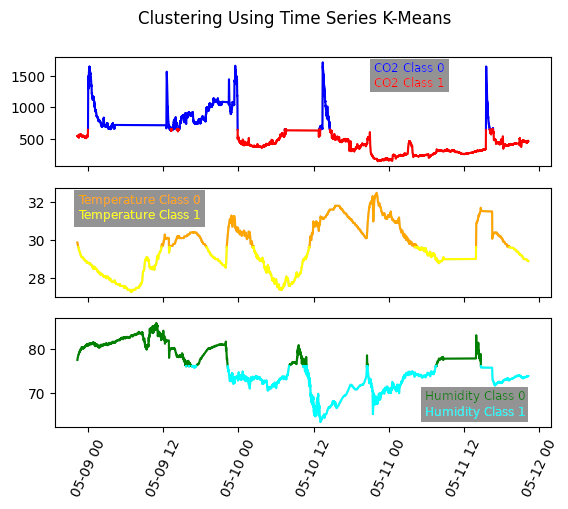
\includegraphics[scale=0.65]{resources/iot-clustering.png}}
      \caption{Time Series KMeans clustering result visualization}
      \label{kmeans}
\end{figure}
